%%%%%%%%%%%%%%%%%%%%%%%%%%%%%%%%%%%%%%%%%
% The Legrand Orange Book
% Structural Definitions File
% Version 3.0 (18/09/2018)
%
% Original author:
% Mathias Legrand (legrand.mathias@gmail.com)
% with modifications by:
% Vel (vel@latextemplates.com)
% with modifications by:
% Alan Rodas Bonjour (alanrodas@gmail.com)
%
% This file has been downloaded from:
% http://www.LaTeXTemplates.com
%
% License:
% CC BY-NC-SA 3.0 (http://creativecommons.org/licenses/by-nc-sa/3.0/)
%
%%%%%%%%%%%%%%%%%%%%%%%%%%%%%%%%%%%%%%%%%

%----------------------------------------------------------------------------------------
%	VARIOUS REQUIRED PACKAGES AND CONFIGURATIONS
%----------------------------------------------------------------------------------------

\usepackage[dvipsnames]{xcolor} % Required for specifying colors by name

\usepackage[top=3cm,bottom=3cm,left=3cm,right=3cm,headsep=10pt,a4paper]{geometry} % Page margins
\usepackage{changepage}

\usepackage{graphicx} % Required for including pictures
\graphicspath{{Imagenes/}} % Specifies the directory where pictures are stored

\usepackage{lipsum} % Inserts dummy text

\usepackage{tikz} % Required for drawing custom shapes

\usepackage[spanish]{babel} % Spanish language/hyphenation

\usepackage[shortlabels]{enumitem} % Customize lists
\setlist{nolistsep} % Reduce spacing between bullet points and numbered lists

\usepackage{booktabs} % Required for nicer horizontal rules in tables

\usepackage[export]{adjustbox} % Allows changing character box alignment

\usepackage{wrapfig}

\usepackage{appendix}
\renewcommand{\appendixname}{Anexo}
\renewcommand{\appendixpagename}{Anexos}
\renewcommand{\appendixtocname}{Anexos}

\usepackage{listings} % Allow code environments with accents

\usepackage{xkeyval} % Allows key value parameters

\usepackage{enumitem} % Allows enumerations with preffix, suffix

%----------------------------------------------------------------------------------------
%	DEFAULT COLORS AND CODE STYLE
%----------------------------------------------------------------------------------------
\definecolor{primary}{RGB}{243,176,25} % Define the primary color used for highlighting throughout the book

\definecolor{codebase}{RGB}{0,0,0}
\definecolor{codecomments}{RGB}{0,120,0}
\definecolor{codekeywords}{RGB}{0,0,120}
\definecolor{codestrings}{RGB}{150,150,0}
\definecolor{codemorekeywords}{RGB}{200,50,50}

\lstset{
    basicstyle=\ttfamily\small,
    numberstyle=\footnotesize,
    numbers=left,
    backgroundcolor=\color{gray!10},
    frame=single,
    tabsize=2,
    rulecolor=\color{codebase!30},
    commentstyle=\color{codecomments},
    keywordstyle=\color{codekeywords},
    stringstyle=\color{codestrings},
    title=\lstname,
    escapeinside={\%(*}{*)},
    breaklines=true,
    breakatwhitespace=true,
    showstringspaces=false,
    framextopmargin=2pt,
    framexbottommargin=2pt,
    framexleftmargin=2pt,
    framexrightmargin=2pt,
    inputencoding=utf8,
    extendedchars=true,
    literate={á}{{\'a}}1 {é}{{\'e}}1 {í}{{\'i}}1 {ó}{{\'o}}1 {ú}{{\'u}}1
             {Á}{{\'A}}1 {É}{{\'E}}1 {Í}{{\'I}}1 {Ó}{{\'O}}1 {Ú}{{\'U}}1
             {ñ}{{\~n}}1 {Ñ}{{\~N}}1 {¿}{{\textquestiondown}}1 {¡}{{\!`}}1
             {©}{{\copyright}}1,
}
\let\origthelstnumber\thelstnumber
\makeatletter
\newcommand*\Suppressnumber{%
  \lst@AddToHook{OnNewLine}{%
    \let\thelstnumber\relax%
     \advance\c@lstnumber-\@ne\relax%
    }%
}

\newcommand*\Reactivatenumber{%
  \lst@AddToHook{OnNewLine}{%
   \let\thelstnumber\origthelstnumber%
   \advance\c@lstnumber\@ne\relax}%
}
\makeatother

\lstdefinelanguage{ini}
{
  showstringspaces=false,
  morestring=[s]{[}{]},
  morecomment=[l]{;},
  moredelim=[l][\color{codebase}]{=},
  stringstyle=\color{codestrings},
  identifierstyle=\color{codekeywords},
}
\lstdefinelanguage{XHTML}
{
  showstringspaces=false,
  morestring=[s]{"}{"},
  morestring=[s]{>}{<},
  morecomment=[s]{!--}{--},
  moredelim=[s][\color{codebase}]{>}{<},
  moredelim=[s][\color{codemorekeywords}]{\ }{=},
  stringstyle=\color{codestrings},
  identifierstyle=\color{codekeywords},
}
\lstdefinelanguage{Markdown}
{
  showstringspaces=false,
  morestring=[s]{`}{`},
  morecomment=[s]{**}{**},
  morecomment=[s]{_}{_},
  moredelim=[s][\color{codebase}]{[}{]}
  keywordstyle = [2]{\color{codekeywords}},
  otherkeywords = {\#},
  morekeywords = [2]{\#},
}
\lstdefinelanguage{CSS}{
  morekeywords={accelerator,align,animation,azimuth,background,
    background-attachment,background-color,background-image,background-position,
    background-position-x,background-position-y,background-repeat,
    behavior,border,border-bottom,border-bottom-color,
    border-bottom-style,border-bottom-width,border-collapse,
    border-color,border-left,border-left-color,border-left-style,
    border-left-width,border-right,border-right-color,
    border-right-style,border-right-width,border-spacing,
    border-style,border-top,border-top-color,border-top-style,
    border-top-width,border-width,bottom,caption-side,clear,
    clip,color,content,counter-increment,counter-reset,cue,
    cue-after,cue-before,cursor,decoration,direction,display,elevation,
    empty-cells,filter,flex,float,font,font-family,font-size,
    font-size-adjust,font-stretch,font-style,font-variant,
    font-weight,height,ime-mode,include-source,justify
    layer-background-color,layer-background-image,layout-flow,
    layout-grid,layout-grid-char,layout-grid-char-spacing,
    layout-grid-line,layout-grid-mode,layout-grid-type,left,
    letter-spacing,line-break,line-height,list-style,
    list-style-image,list-style-position,list-style-type,margin,
    margin-bottom,margin-left,margin-right,margin-top,
    marker-offset,marks,max-height,max-width,min-height,
    min-width,-moz-binding,-moz-border-radius,
    -moz-border-radius-topleft,-moz-border-radius-topright,
    -moz-border-radius-bottomright,-moz-border-radius-bottomleft,
    -moz-border-top-colors,-moz-border-right-colors,
    -moz-border-bottom-colors,-moz-border-left-colors,-moz-opacity,
    -moz-outline,-moz-outline-color,-moz-outline-style,
    -moz-outline-width,-moz-user-focus,-moz-user-input,
    -moz-user-modify,-moz-user-select,orphans,outline,
    outline-color,outline-style,outline-width,overflow,
    overflow-X,overflow-Y,padding,padding-bottom,padding-left,
    padding-right,padding-top,page,page-break-after,
    page-break-before,page-break-inside,pause,pause-after,
    pause-before,pitch,pitch-range,play-during,position,quotes,
    radius,-replace,richness,right,ruby-align,ruby-overhang,
    ruby-position,-set-link-source,size,speak,speak-header,
    speak-numeral,speak-punctuation,speech-rate,stress,
    scrollbar-arrow-color,scrollbar-base-color,
    scrollbar-dark-shadow-color,scrollbar-face-color,
    scrollbar-highlight-color,scrollbar-shadow-color,
    scrollbar-3d-light-color,scrollbar-track-color,table-layout,
    text,text-align,text-align-last,text-decoration,text-indent,
    text-justify,text-overflow,text-shadow,text-transform,
    text-autospace,text-kashida-space,text-underline-position,top,
    unicode-bidi,-use-link-source,vertical-align,visibility,
    voice-family,volume,weight,white-space,widows,width,word-break,
    word-spacing,word-wrap,writing-mode,z-index,zoom},
  morestring=[s]{:}{;},
  sensitive,
  morecomment=[s]{/*}{*/}
}
%----------------------------------------------------------------------------------------
%	FONTS
%----------------------------------------------------------------------------------------

\usepackage{avant} % Use the Avantgarde font for headings
%\usepackage{times} % Use the Times font for headings
\usepackage{mathptmx} % Use the Adobe Times Roman as the default text font together with math symbols from the Sym­bol, Chancery and Com­puter Modern fonts

\usepackage{microtype} % Slightly tweak font spacing for aesthetics
\usepackage[utf8]{inputenc} % Required for including letters with accents
\usepackage[T1]{fontenc} % Use 8-bit encoding that has 256 glyphs

%----------------------------------------------------------------------------------------
%	BIBLIOGRAPHY AND INDEX
%----------------------------------------------------------------------------------------

\usepackage{csquotes}
\usepackage[style=numeric,citestyle=numeric,autocite=superscript,sorting=none,sortcites=false,autopunct=true,autolang=other,hyperref=true,abbreviate=false,backref=true,backend=biber]{biblatex}
\addbibresource{bibliography.bib} % BibTeX bibliography file
\defbibheading{bibempty}{}

\usepackage{calc} % For simpler calculation - used for spacing the index letter headings correctly
\usepackage{makeidx} % Required to make an index
\makeindex % Tells LaTeX to create the files required for indexing

%----------------------------------------------------------------------------------------
%	GENERAL STYLES USED THROUGH THE DOCUMENT
%----------------------------------------------------------------------------------------

% \setlength{\parindent}{4em}
% \setlength{\parskip}{0.5em}
% \renewcommand{\baselinestretch}{1.5}

%----------------------------------------------------------------------------------------
%	DEFINITIONS USED THROUGH THE DOCUMENT (USER SHOULD SET THIS)
%----------------------------------------------------------------------------------------

\makeatletter

\def\@subtitle{\relax}
\newcommand{\subtitle}[1]{\gdef\@subtitle{#1}}

\def\@department{\relax}
\newcommand{\department}[1]{\gdef\@department{#1}}

\def\@institution{\relax}
\newcommand{\institution}[1]{\gdef\@institution{#1}}

\def\@version{\relax}
\newcommand{\version}[1]{\gdef\@version{#1}}

\def\@rprimary{\relax}
\def\@gprimary{\relax}
\def\@bprimary{\relax}
\newcommand{\primarycolor}[3]{
    \definecolor{primary}{RGB}{#1,#2,#3}
}

\makeatother

%----------------------------------------------------------------------------------------
%	CUSTOM IMAGES
%----------------------------------------------------------------------------------------

\newcommand{\image}[4][0.75]{
    \begin{figure}[ht]
        \centering
        \includegraphics[width=#1\textwidth,keepaspectratio]{#2}
        \parbox{#1\textwidth}{
            \small
            \begin{flushright}
                #3\\
                \color{gray}{#4}
            \end{flushright}
            \normalsize
        }
    \end{figure}
}

%----------------------------------------------------------------------------------------

\newcommand{\wrapimage}[5][0.35]{
    \begin{wrapfigure}{#5}{#1\textwidth}
        \centering
        \includegraphics[width=#1\textwidth,keepaspectratio]{#2}
        \parbox{#1\textwidth}{
            \small
            \begin{flushright}
                #3\\
                \color{gray}{#4}
            \end{flushright}
            \normalsize
        }
    \end{wrapfigure}
}

\newcommand{\wraprimage}[4][0.35]{\wrapimage[#1]{#2}{#3}{#4}{R}}
\newcommand{\wraplimage}[4][0.35]{\wrapimage[#1]{#2}{#3}{#4}{L}}

%----------------------------------------------------------------------------------------
%	MAIN TABLE OF CONTENTS
%----------------------------------------------------------------------------------------

\usepackage{titletoc} % Required for manipulating the table of contents

\contentsmargin{0cm} % Removes the default margin

% Override maketitle
\makeatletter
\def\maketitle{%
    \begingroup
    \thispagestyle{empty}
    \begin{tikzpicture}[remember picture,overlay]
    \node[inner sep=0pt] (background) at (current page.center) {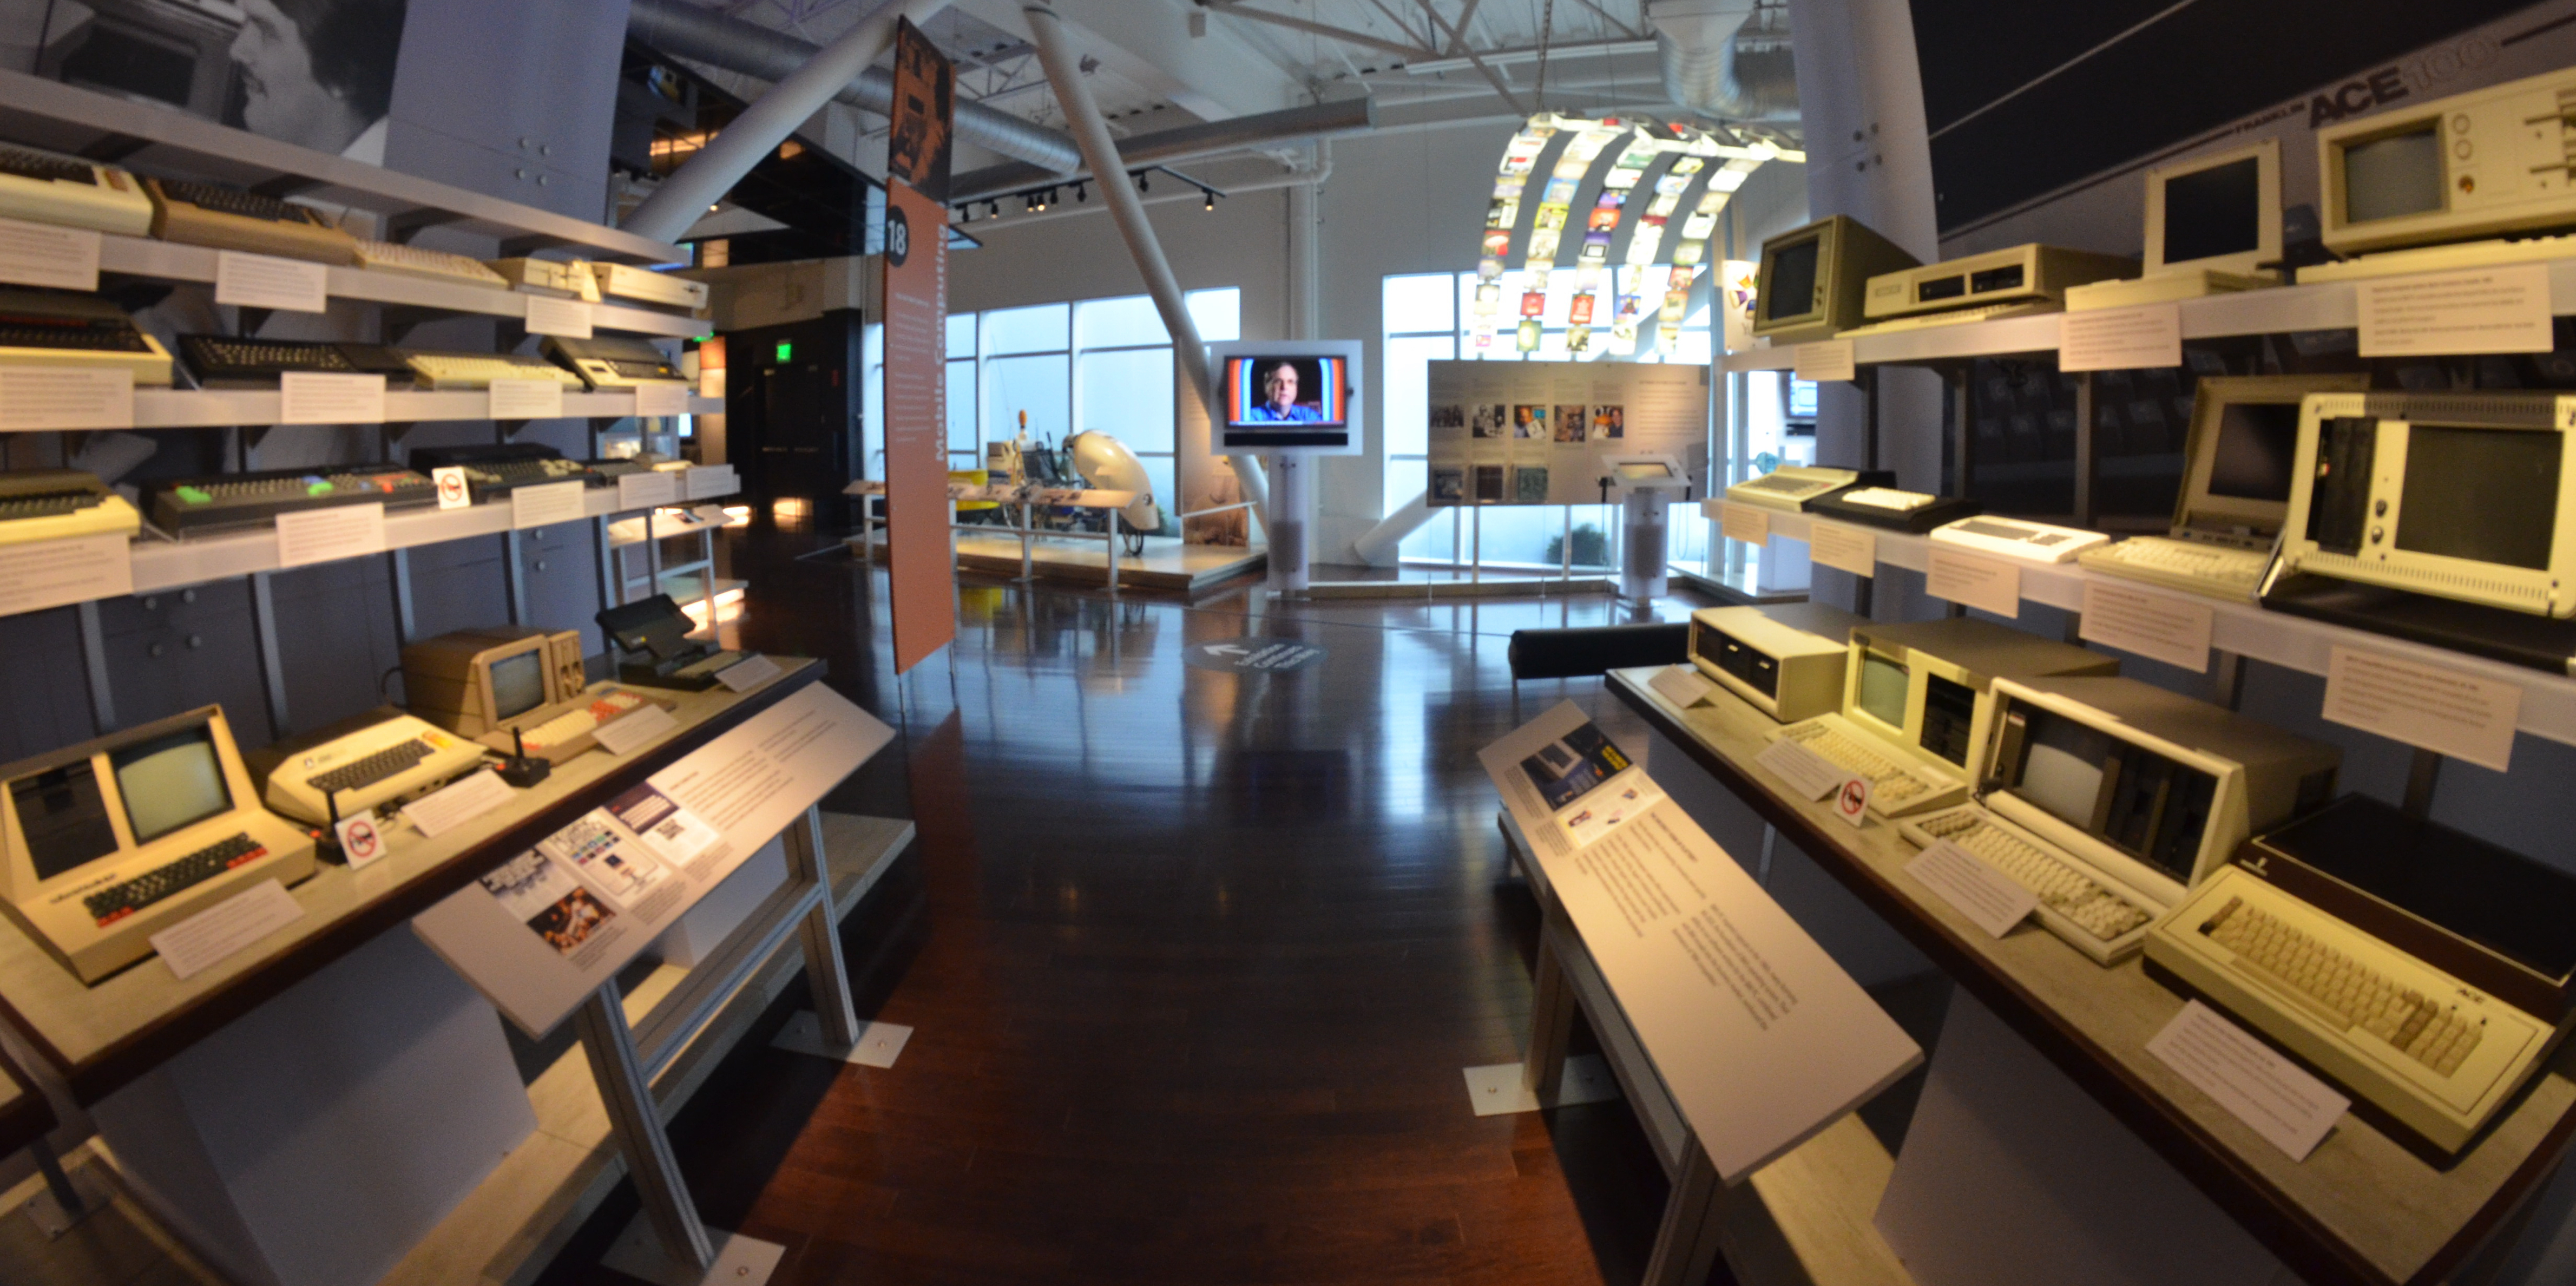
\includegraphics[width=\paperwidth]{cover}};
    \draw (current page.center) node [fill=primary, text=white, text opacity=1,inner sep=1cm]{\centering\bfseries\sffamily\parbox[c][][t]{\paperwidth}{\centering
    {\Large \@institution}\\[3pt] % Institution
    {\Huge \@title}\\[25pt] % Book title
    {\huge \@subtitle}\\[15pt] % Subtitle
    {\Large por \@author}\\[20pt] % Author
    {\large Ver. \@version \quad (\@date)}}}; % Version and date
    \end{tikzpicture}
    \vfill
    \endgroup
}
\makeatother

% Part text styling
\titlecontents{part}[0cm]
{\addvspace{20pt}\centering\large\bfseries}
{}
{}
{}

% Chapter text styling
\titlecontents{chapter}[1.25cm] % Indentation
{\addvspace{12pt}\large\sffamily\bfseries} % Spacing and font options for chapters
{\color{primary!60}\contentslabel[\Large\thecontentslabel]{1.25cm}\color{primary}} % Chapter number
{\color{primary}}
{\color{primary!60}\normalsize\;\titlerule*[.5pc]{.}\;\thecontentspage} % Page number

% Section text styling
\titlecontents{section}[1.25cm] % Indentation
{\addvspace{3pt}\sffamily\bfseries} % Spacing and font options for sections
{\contentslabel[\thecontentslabel]{1.25cm}} % Section number
{}
{\hfill\color{black}\thecontentspage} % Page number
[]

% Subsection text styling
\titlecontents{subsection}[1.25cm] % Indentation
{\addvspace{1pt}\sffamily\small} % Spacing and font options for subsections
{\contentslabel[\thecontentslabel]{1.25cm}} % Subsection number
{}
{\ \titlerule*[.5pc]{.}\;\thecontentspage} % Page number
[]

% List of figures
\titlecontents{figure}[0em]
{\addvspace{-5pt}\sffamily}
{\thecontentslabel\hspace*{1em}}
{}
{\ \titlerule*[.5pc]{.}\;\thecontentspage}
[]

% List of tables
\titlecontents{table}[0em]
{\addvspace{-5pt}\sffamily}
{\thecontentslabel\hspace*{1em}}
{}
{\ \titlerule*[.5pc]{.}\;\thecontentspage}
[]

%----------------------------------------------------------------------------------------
%	MINI TABLE OF CONTENTS IN PART HEADS
%----------------------------------------------------------------------------------------

% Chapter text styling
\titlecontents{lchapter}[0em] % Indenting
{\addvspace{15pt}\large\sffamily\bfseries} % Spacing and font options for chapters
{\color{primary}\contentslabel[\Large\thecontentslabel]{1.25cm}\color{primary}} % Chapter number
{}
{\color{primary}\normalsize\sffamily\bfseries\;\titlerule*[.5pc]{.}\;\thecontentspage} % Page number

% Section text styling
\titlecontents{lsection}[0em] % Indenting
{\sffamily\small} % Spacing and font options for sections
{\contentslabel[\thecontentslabel]{1.25cm}} % Section number
{}
{}

% Subsection text styling
\titlecontents{lsubsection}[.5em] % Indentation
{\normalfont\footnotesize\sffamily} % Font settings
{}
{}
{}

%----------------------------------------------------------------------------------------
%	PAGE HEADERS
%----------------------------------------------------------------------------------------

\usepackage{fancyhdr} % Required for header and footer configuration

\pagestyle{fancy}
\renewcommand{\chaptermark}[1]{\markboth{\sffamily\normalsize\bfseries\chaptername\ \thechapter.\ #1}{}} % Chapter text font settings
\renewcommand{\sectionmark}[1]{\markright{\sffamily\normalsize\thesection\hspace{5pt}#1}{}} % Section text font settings
\fancyhf{} \fancyhead[LE,RO]{\sffamily\normalsize\thepage} % Font setting for the page number in the header
\fancyhead[LO]{\rightmark} % Print the nearest section name on the left side of odd pages
\fancyhead[RE]{\leftmark} % Print the current chapter name on the right side of even pages
\renewcommand{\headrulewidth}{0.5pt} % Width of the rule under the header
\addtolength{\headheight}{2.5pt} % Increase the spacing around the header slightly
\renewcommand{\footrulewidth}{0pt} % Removes the rule in the footer
\fancypagestyle{plain}{\fancyhead{}\renewcommand{\headrulewidth}{0pt}} % Style for when a plain pagestyle is specified

% Removes the header from odd empty pages at the end of chapters
\makeatletter
\renewcommand{\cleardoublepage}{
\clearpage\ifodd\c@page\else
\hbox{}
\vspace*{\fill}
\thispagestyle{empty}
\newpage
\fi}

%----------------------------------------------------------------------------------------
%	THEOREM STYLES
%----------------------------------------------------------------------------------------

\usepackage{amsmath,amsfonts,amssymb,amsthm} % For math equations, theorems, symbols, etc

\newcommand{\intoo}[2]{\mathopen{]}#1\,;#2\mathclose{[}}
\newcommand{\ud}{\mathop{\mathrm{{}d}}\mathopen{}}
\newcommand{\intff}[2]{\mathopen{[}#1\,;#2\mathclose{]}}
\newtheorem{notation}{Notación}[chapter]

% Boxed/framed environments
\newtheoremstyle{primarynumbox}% % Theorem style name
{0pt}% Space above
{0pt}% Space below
{\normalfont}% % Body font
{}% Indent amount
{\small\bf\sffamily\color{primary}}% % Theorem head font
{\;}% Punctuation after theorem head
{0.25em}% Space after theorem head
{\small\sffamily\color{primary}\thmname{#1}\nobreakspace\thmnumber{\@ifnotempty{#1}{}\@upn{#2}}% Theorem text (e.g. Theorem 2.1)
\thmnote{\nobreakspace\the\thm@notefont\sffamily\bfseries\color{black}---\nobreakspace#3.}} % Optional theorem note
\renewcommand{\qedsymbol}{$\blacksquare$}% Optional qed square

\newtheoremstyle{blacknumex}% Theorem style name
{5pt}% Space above
{5pt}% Space below
{\normalfont}% Body font
{} % Indent amount
{\small\bf\sffamily}% Theorem head font
{\;}% Punctuation after theorem head
{0.25em}% Space after theorem head
{\small\sffamily{\tiny\ensuremath{\textcolor{primary}{\blacksquare}}}\nobreakspace\thmname{#1}\nobreakspace\thmnumber{\@ifnotempty{#1}{}\@upn{#2}}\\% Theorem text (e.g. Theorem 2.1)
\thmnote{\nobreakspace\the\thm@notefont\sffamily\bfseries---\nobreakspace#3.}}% Optional theorem note

\newtheoremstyle{blacknumbox} % Theorem style name
{0pt}% Space above
{0pt}% Space below
{\normalfont}% Body font
{}% Indent amount
{\small\bf\sffamily}% Theorem head font
{\;}% Punctuation after theorem head
{0.25em}% Space after theorem head
{\small\sffamily\thmname{#1}\nobreakspace\thmnumber{\@ifnotempty{#1}{}\@upn{#2}}% Theorem text (e.g. Theorem 2.1)
\thmnote{\nobreakspace\the\thm@notefont\sffamily\bfseries---\nobreakspace#3.}}% Optional theorem note

% Non-boxed/non-framed environments
\newtheoremstyle{primarynum}% % Theorem style name
{5pt}% Space above
{5pt}% Space below
{\normalfont}% % Body font
{}% Indent amount
{\small\bf\sffamily\color{primary}}% % Theorem head font
{\;}% Punctuation after theorem head
{0.25em}% Space after theorem head
{\small\sffamily\color{primary}\thmname{#1}\nobreakspace\thmnumber{\@ifnotempty{#1}{}\@upn{#2}}% Theorem text (e.g. Theorem 2.1)
\thmnote{\nobreakspace\the\thm@notefont\sffamily\bfseries\color{black}---\nobreakspace#3.}} % Optional theorem note
\renewcommand{\qedsymbol}{$\blacksquare$}% Optional qed square
\makeatother

% Defines the theorem text style for each type of theorem to one of the three styles above
\newcounter{dummy}
\numberwithin{dummy}{section}
\theoremstyle{primarynumbox}
\newtheorem{theoremeT}[dummy]{Teorema}
\newtheorem{problem}{Problema}[chapter]
\newtheorem{exerciseT}{Ejercicio}[chapter]
\theoremstyle{blacknumex}
\newtheorem{exampleT}{Ejemplo}[chapter]
\theoremstyle{blacknumbox}
\newtheorem{vocabulary}{Vocabulario}[chapter]
\newtheorem{definitionT}{Definición}[chapter]
\newtheorem{corollaryT}[dummy]{Corolario}
\theoremstyle{primarynum}
\newtheorem{proposition}[dummy]{Proposición}

%----------------------------------------------------------------------------------------
%	DEFINITION OF COLORED BOXES
%----------------------------------------------------------------------------------------

\RequirePackage[framemethod=default]{mdframed} % Required for creating the theorem, definition, exercise and corollary boxes

% Theorem box
\newmdenv[skipabove=7pt,
skipbelow=7pt,
backgroundcolor=black!5,
linecolor=primary,
innerleftmargin=5pt,
innerrightmargin=5pt,
innertopmargin=5pt,
leftmargin=0cm,
rightmargin=0cm,
innerbottommargin=5pt]{tBox}

% Exercise box
\newmdenv[skipabove=5pt,
skipbelow=7pt,
rightline=false,
leftline=true,
topline=false,
bottomline=false,
backgroundcolor=primary!10,
linecolor=primary,
innerleftmargin=5pt,
innerrightmargin=5pt,
innertopmargin=10pt,
innerbottommargin=5pt,
leftmargin=0cm,
rightmargin=0cm,
linewidth=4pt]{eBox}

% Definition box
\newmdenv[skipabove=17pt,
skipbelow=7pt,
rightline=false,
leftline=true,
topline=false,
bottomline=false,
linecolor=primary,
innerleftmargin=5pt,
innerrightmargin=5pt,
innertopmargin=10pt,
innerbottommargin=5pt,
leftmargin=0cm,
rightmargin=0cm,
linewidth=4pt]{dBox}

% Corollary box
\newmdenv[skipabove=7pt,
skipbelow=7pt,
rightline=false,
leftline=true,
topline=false,
bottomline=false,
linecolor=gray,
backgroundcolor=black!5,
innerleftmargin=5pt,
innerrightmargin=5pt,
innertopmargin=5pt,
leftmargin=0cm,
rightmargin=0cm,
linewidth=4pt,
innerbottommargin=5pt]{cBox}

% Creates an environment for each type of theorem and assigns it a theorem text style from the "Theorem Styles" section above and a colored box from above
\newenvironment{theorem}{\begin{tBox}\begin{theoremeT}}{\end{theoremeT}\end{tBox}}
\newenvironment{exercise}{\begin{eBox}\begin{exerciseT}}{\hfill{\color{primary}\tiny\ensuremath{\blacksquare}}\end{exerciseT}\end{eBox}}
\newenvironment{knowwhat}[1][Sabías qué]{\begin{eBox}\textcolor{primary}{\textbf{#1}}\\}{\hfill{\color{primary}}\end{eBox}}
\newenvironment{definition}{\begin{dBox}\begin{definitionT}}{\end{definitionT}\end{dBox}}
\newenvironment{example}{\begin{exampleT}}{\hfill{\tiny\ensuremath{\blacksquare}}\end{exampleT}}
\newenvironment{corollary}{\begin{cBox}\begin{corollaryT}}{\end{corollaryT}\end{cBox}}
\newenvironment{solution}{\vspace*{10pt}}{\vspace*{30pt}}

%----------------------------------------------------------------------------------------
%	REMARK ENVIRONMENT
%----------------------------------------------------------------------------------------

\newenvironment{remark}{\par\vspace{10pt}\small % Vertical white space above the remark and smaller font size
\begin{list}{}{
\leftmargin=35pt % Indentation on the left
\rightmargin=25pt}\item\ignorespaces % Indentation on the right
\makebox[-2.5pt]{\begin{tikzpicture}[overlay]
\node[draw=primary!60,line width=1pt,circle,fill=primary!25,font=\sffamily\bfseries,inner sep=2pt,outer sep=0pt] at (-15pt,0pt){\textcolor{primary}{!}};\end{tikzpicture}} % Orange R in a circle
\advance\baselineskip -1pt}{\end{list}\vskip5pt} % Tighter line spacing and white space after remark

\newenvironment{hint}{\par\vspace{10pt}\small % Vertical white space above the remark and smaller font size
\begin{list}{}{
\leftmargin=35pt % Indentation on the left
\rightmargin=25pt}\item\ignorespaces % Indentation on the right
\makebox[-2.5pt]{\begin{tikzpicture}[overlay]
\node[draw=yellow!60,line width=1pt,circle,fill=yellow!25,font=\sffamily\bfseries,inner sep=2pt,outer sep=0pt] at (-15pt,0pt){\textcolor{yellow}{X}};\end{tikzpicture}} % Orange R in a circle
\advance\baselineskip -1pt}{\end{list}\vskip5pt} % Tighter line spacing and white space after remark

\newenvironment{question}{\par\vspace{10pt}\small % Vertical white space above the remark and smaller font size
\begin{list}{}{
\leftmargin=35pt % Indentation on the left
\rightmargin=25pt}\item\ignorespaces % Indentation on the right
\makebox[-2.5pt]{\begin{tikzpicture}[overlay]
\node[draw=blue!60,line width=1pt,circle,fill=blue!25,font=\sffamily\bfseries,inner sep=2pt,outer sep=0pt] at (-15pt,0pt){\textcolor{blue}{?}};\end{tikzpicture}} % Orange R in a circle
\advance\baselineskip -1pt}{\end{list}\vskip5pt} % Tighter line spacing and white space after remark

\newenvironment{money}{\par\vspace{10pt}\small % Vertical white space above the remark and smaller font size
\begin{list}{}{
\leftmargin=35pt % Indentation on the left
\rightmargin=25pt}\item\ignorespaces % Indentation on the right
\makebox[-2.5pt]{\begin{tikzpicture}[overlay]
\node[draw=green!60,line width=1pt,circle,fill=green!25,font=\sffamily\bfseries,inner sep=2pt,outer sep=0pt] at (-15pt,0pt){\textcolor{green}{\$}};\end{tikzpicture}} % Orange R in a circle
\advance\baselineskip -1pt}{\end{list}\vskip5pt} % Tighter line spacing and white space after remark


%----------------------------------------------------------------------------------------
%	SECTION NUMBERING IN THE MARGIN
%----------------------------------------------------------------------------------------

\makeatletter
\renewcommand{\@seccntformat}[1]{\llap{\textcolor{primary}{\csname the#1\endcsname}\hspace{1em}}}
\renewcommand{\section}{\@startsection{section}{1}{\z@}
{-4ex \@plus -1ex \@minus -.4ex}
{1ex \@plus.2ex }
{\normalfont\large\sffamily\bfseries}}
\renewcommand{\subsection}{\@startsection {subsection}{2}{\z@}
{-3ex \@plus -0.1ex \@minus -.4ex}
{0.5ex \@plus.2ex }
{\normalfont\sffamily\bfseries}}
\renewcommand{\subsubsection}{\@startsection {subsubsection}{3}{\z@}
{-2ex \@plus -0.1ex \@minus -.2ex}
{.2ex \@plus.2ex }
{\normalfont\small\sffamily\bfseries}}
\renewcommand\paragraph{\@startsection{paragraph}{4}{\z@}
{-2ex \@plus-.2ex \@minus .2ex}
{.1ex}
{\normalfont\small\sffamily\bfseries}}

%----------------------------------------------------------------------------------------
%	PART HEADINGS
%----------------------------------------------------------------------------------------

% numbered part in the table of contents
\newcommand{\@mypartnumtocformat}[2]{%
\setlength\fboxsep{0pt}%
\noindent\colorbox{primary!20}{\strut\parbox[c][.7cm]{\ecart}{\color{primary!70}\Large\sffamily\bfseries\centering#1}}\hskip\esp\colorbox{primary!40}{\strut\parbox[c][.7cm]{\linewidth-\ecart-\esp}{\Large\sffamily\centering#2}}}%
%%%%%%%%%%%%%%%%%%%%%%%%%%%%%%%%%%
% unnumbered part in the table of contents
\newcommand{\@myparttocformat}[1]{%
\setlength\fboxsep{0pt}%
\noindent\colorbox{primary!40}{\strut\parbox[c][.7cm]{\linewidth}{\Large\sffamily\centering#1}}}%
%%%%%%%%%%%%%%%%%%%%%%%%%%%%%%%%%%
\newlength\esp
\setlength\esp{4pt}
\newlength\ecart
\setlength\ecart{1.2cm-\esp}
\newcommand{\thepartimage}{}%
\newcommand{\partimage}[1]{\renewcommand{\thepartimage}{#1}}%
\def\@part[#1]#2{%
\ifnum \c@secnumdepth >-2\relax%
\refstepcounter{part}%
\addcontentsline{toc}{part}{\texorpdfstring{\protect\@mypartnumtocformat{\thepart}{#1}}{\partname~\thepart\ ---\ #1}}
\else%
\addcontentsline{toc}{part}{\texorpdfstring{\protect\@myparttocformat{#1}}{#1}}%
\fi%
\startcontents%
\markboth{}{}%
{\thispagestyle{empty}%
\begin{tikzpicture}[remember picture,overlay]%
\node at (current page.north west){\begin{tikzpicture}[remember picture,overlay]%
\fill[primary!20](0cm,0cm) rectangle (\paperwidth,-\paperheight);
\node[anchor=north] at (4cm,-3.25cm){\color{primary!40}\fontsize{220}{100}\sffamily\bfseries\thepart};
\node[anchor=south east] at (\paperwidth-1cm,-\paperheight+1cm){\parbox[t][][t]{8.5cm}{
\printcontents{l}{0}{\setcounter{tocdepth}{1}}%
}};
\node[anchor=north east] at (\paperwidth-1.5cm,-3.25cm){\parbox[t][][t]{15cm}{\strut\raggedleft\color{white}\fontsize{30}{30}\sffamily\bfseries#2}};
\end{tikzpicture}};
\end{tikzpicture}}%
\@endpart}
\def\@spart#1{%
\startcontents%
\phantomsection
{\thispagestyle{empty}%
\begin{tikzpicture}[remember picture,overlay]%
\node at (current page.north west){\begin{tikzpicture}[remember picture,overlay]%
\fill[primary!20](0cm,0cm) rectangle (\paperwidth,-\paperheight);
\node[anchor=north east] at (\paperwidth-1.5cm,-3.25cm){\parbox[t][][t]{15cm}{\strut\raggedleft\color{white}\fontsize{30}{30}\sffamily\bfseries#1}};
\end{tikzpicture}};
\end{tikzpicture}}
\addcontentsline{toc}{part}{\texorpdfstring{%
\setlength\fboxsep{0pt}%
\noindent\protect\colorbox{primary!40}{\strut\protect\parbox[c][.7cm]{\linewidth}{\Large\sffamily\protect\centering #1\quad\mbox{}}}}{#1}}%
\@endpart}
\def\@endpart{\vfil\newpage
\if@twoside
\if@openright
\null
\thispagestyle{empty}%
\newpage
\fi
\fi
\if@tempswa
\twocolumn
\fi}

%----------------------------------------------------------------------------------------
%	CHAPTER HEADINGS
%----------------------------------------------------------------------------------------

% A switch to conditionally include a picture, implemented by  Christian Hupfer
\newif\ifusechapterimage
\usechapterimagetrue
\newcommand{\thechapterimage}{}%
\newcommand{\thechapterimagedescription}{}%
\newcommand{\thechapterimageauthor}{}%
\newcommand{\chapterimage}[1]{\ifusechapterimage\renewcommand{\thechapterimage}{#1}\fi}%
\newcommand{\chapterimagedescription}[1]{\ifusechapterimage\renewcommand{\thechapterimagedescription}{#1}\fi}%
\newcommand{\chapterimageauthor}[1]{\ifusechapterimage\renewcommand{\thechapterimageauthor}{#1}\fi}%
\newcommand{\autodot}{.}
\def\@makechapterhead#1{%
{\parindent \z@ \raggedright \normalfont
\ifnum \c@secnumdepth >\m@ne
\if@mainmatter
\begin{tikzpicture}[remember picture,overlay]
\node at (current page.north west)
{\begin{tikzpicture}[remember picture,overlay]
\node[anchor=north west,inner sep=0pt] at (0,0) {\ifusechapterimage\includegraphics[width=\paperwidth]{\thechapterimage}\fi};
\draw[anchor=west] (\Gm@lmargin,-9cm) node [line width=2pt,rounded corners=15pt,draw=primary,fill=white,fill opacity=0.5,inner sep=15pt]{\strut\makebox[22cm]{}};
\draw[anchor=west] (\Gm@lmargin+.3cm,-9cm) node {\huge\sffamily\bfseries\color{black}\thechapter\autodot~#1\strut};
\draw[anchor=east] (\Gm@lmargin+17.5cm,-11.5cm) node {\ifusechapterimage{\raggedright\color{gray}\thechapterimagedescription\autodot}\fi};
\draw[anchor=east] (\Gm@lmargin+17.5cm,-12cm) node {\ifusechapterimage{\raggedright\color{gray}\thechapterimageauthor\autodot}\fi};
\end{tikzpicture}};
\end{tikzpicture}
\else
\begin{tikzpicture}[remember picture,overlay]
\node at (current page.north west)
{\begin{tikzpicture}[remember picture,overlay]
\node[anchor=north west,inner sep=0pt] at (0,0) {\ifusechapterimage\includegraphics[width=\paperwidth]{\thechapterimage}\fi};
\draw[anchor=west] (\Gm@lmargin,-9cm) node [line width=2pt,rounded corners=15pt,draw=primary,fill=white,fill opacity=0.5,inner sep=15pt]{\strut\makebox[22cm]{}};
\draw[anchor=west] (\Gm@lmargin+.3cm,-9cm) node {\huge\sffamily\bfseries\color{black}#1\strut};
%\draw[anchor=east] (\Gm@lmargin+17.5cm,-11cm) node {\ifusechapterimage{\raggedright\color{gray}\thechapterimagedescription\autodot}\fi};
%\draw[anchor=east] (\Gm@lmargin+17.5cm,-11.5cm) node {\ifusechapterimage{\raggedright\color{gray}\thechapterimageauthor\autodot}\fi};
\end{tikzpicture}};
\end{tikzpicture}
\fi\fi\par\vspace*{270\p@}}}

%-------------------------------------------

\def\@makeschapterhead#1{%
\begin{tikzpicture}[remember picture,overlay]
\node at (current page.north west)
{\begin{tikzpicture}[remember picture,overlay]
\node[anchor=north west,inner sep=0pt] at (0,0) {\ifusechapterimage\includegraphics[width=\paperwidth]{\thechapterimage}\fi};
\draw[anchor=west] (\Gm@lmargin,-9cm) node [line width=2pt,rounded corners=15pt,draw=primary,fill=white,fill opacity=0.5,inner sep=15pt]{\strut\makebox[22cm]{}};
\draw[anchor=west] (\Gm@lmargin+.3cm,-9cm) node {\huge\sffamily\bfseries\color{black}#1\strut};
\draw[anchor=east] (\Gm@lmargin+17.5cm,-11.5cm) node {\ifusechapterimage{\raggedright\color{gray}\thechapterimagedescription\autodot}\fi};
\draw[anchor=east] (\Gm@lmargin+17.5cm,-12cm) node {\ifusechapterimage{\raggedright\color{gray}\thechapterimageauthor\autodot}\fi};
\end{tikzpicture}};
\end{tikzpicture}
\par\vspace*{270\p@}}
\makeatother

%----------------------------------------------------------------------------------------
%	HYPERLINKS IN THE DOCUMENTS
%----------------------------------------------------------------------------------------

\usepackage{hyperref}
\hypersetup{hidelinks,backref=true,pagebackref=true,hyperindex=true,colorlinks=false,breaklinks=true,urlcolor= primary,bookmarks=true,bookmarksopen=false,pdftitle={Title},pdfauthor={Author}}
\usepackage{bookmark}
\bookmarksetup{
open,
numbered,
addtohook={%
\ifnum\bookmarkget{level}=0 % chapter
\bookmarksetup{bold}%
\fi
\ifnum\bookmarkget{level}=-1 % part
\bookmarksetup{color=primary,bold}%
\fi
}
}

%----------------------------------------------------------------------------------------
%	SPECIAL TRANSLATIONS
%----------------------------------------------------------------------------------------
\addto\extrasspanish{%
\def\partautorefname{Unidad}%
\def\appendixautorefname{Anexo}%
}

%----------------------------------------------------------------------------------------
%	SPECIAL INDENTS AND LINES
%----------------------------------------------------------------------------------------
\newcommand{\crline}[2][10pt]{
    \noindent #2

    \vspace{#1}
}

\newcounter{sindentwidth}
\newcounter{dindentwidth}
\setcounter{sindentwidth}{16}
\setcounter{dindentwidth}{32}

\newcommand{\sindent}{\noindent\hspace*{\value{sindentwidth} pt}}
\newcommand{\dindent}{\noindent\hspace*{\value{dindentwidth} pt}}

%----------------------------------------------------------------------------------------
%	EMOJI IMAGES SUPPORT (IMAGES NOT PROVIDED)
%----------------------------------------------------------------------------------------
\newcommand{\emoji}[1]{%
  \includegraphics[width=1em,valign=t,raise=-0.1em]{#1}%
}

%----------------------------------------------------------------------------------------
%	DARK MODE SUPPORT
%----------------------------------------------------------------------------------------
\newcommand{\darkmode}{
  \pagecolor{black!80}
  \color{white!30}
}
